
% this was used for first submission 
\documentclass{acm_proc_article-sp} 
%\documentclass{sig-alternate-2013}
\usepackage{url}
\usepackage{verbatim}
\usepackage{subfigure}

 % \clubpenalty=10000 
 % \widowpenalty = 10000 

\pdfpagewidth=8.5in
\pdfpageheight=11in

\title{ Estimating User-Produced-Multimedia Classification Performance Efficiently with Python }

\numberofauthors{5}
\author{
\alignauthor 
Peter Birsinger\\
       \affaddr{UC Berkeley}\\
       \email{peterbir@eecs.berkeley.edu}
\alignauthor 
Benjamin Elizalde\\
       \affaddr{UC Berkeley}\\
       \email{benmael@icsi}%.berkeley.edu}
\alignauthor 
Karl Ni\\
       \affaddr{UC Berkeley}\\
       \email{ni4@llnl.gov}
\and
\alignauthor 
Gerald Friedland\\
       \affaddr{UC Berkeley}\\
       \email{fractor@icsi}%.berkeley.edu}
\alignauthor 
Armando Fox\\
       \affaddr{UC Berkeley}\\
       \email{fox@cs.berkeley.edu}
}

\begin{document}

\maketitle


\begin{abstract}
When developing a multimedia classification system in preparation for an evaluation such as TRECVID MED or MediaEval, one typically must estimate the error on the evaluation data set from the performance on the development data set, a task made increasingly important with user-produced videos that often lack structure and have high acoustic variability. 
Statistical bootsrapping reveals the uncertainty of the estimate of a classifier's performance, yet with today's large multimedia datasets, bootstrapping applications, particularly when written in common productivity languages such as Python or Matlab, can become essentially intractable, as we later show.

To combat this, we propose here a methodology to efficiently estimate classifier performance that relies on the ability to generate distributed bootstrapping applications from serial Python. 
Utilizing an already made Domain-Specific Embedded Language (DSEL) and corresponding DSEL compiler \cite{pbirsinger2013} made with the SEJITS (Selective Embedded Just-In-Time Specialization) approach \cite{Kamil:EECS-2013-1}, we describe a bootstrapping application in Python to evaluate a multimedia classifier's performance and   automatically generate distributed code scalable to demanding data sizes and computational workloads. 
With this methodology we obtain reasonable bounds for classifier performance predictions on user-produced videos from the 2013 TRECVID MED corpus, showing that reasonbly estimating performance on such data is possible. 
We then demonstrate the newfound accessibility to such computations for non-performance programmers by exposing the orders of magnitude speedup obtained over the native Python code.
\end{abstract} 

% Statistical bootsrapping reveals the uncertainty of the estimate of a classifier's performance, yet often requires considerable computational resources, a problem compounded by today's sizable multimedia datasets.
% We show that large bootstrapping multimedia applications, particularly when written in common productivity languages such as Python or Matlab, can become essentially intractable. 

% \category{D.1.3}{Programming Techniques}{Concurrent Programming}[distributed programming]
% \category{D.3.2}{Programming Langauges}{Language Classifications}[concurrent, distributed, and parallel languages]

\keywords{Multimedia classification; bootstrapping; SEJITS}

\section{Introduction}
User-produced multimedia data has grown abundant recently with the ubiquity of recording devices and online sharing websites, yet these files must be able to be retrieved easily for them to have value. 
Video detection systems that analyze and fetch multimedia files solve this problem of video event detection, or the classification of videos with regards to semantically defined events (e.g. marriage proposals or changing a car tire). 

Preparing such multimedia classification systems often requires estimating the system's performance on unseen consumer-produced videos based on its performance on known consumer-produced videos. Fortunately, speculation of classifier performance is a well understood problem \cite{fukunaga1989estimation}. 
Extensive investigation of bootstrapping and its variations \cite{efron1979bootstrap,jain1987bootstrap, chernick1985application, sahiner2008classifier} has identified bootstrapping as a prime, ableit not perfect \cite{isaksson2008cross},
solution to this problem. We focus, however, on using bootstrapping to estimate the performance of specifically multimedia classifiers, and doing so efficiently for large applications.

When dealing with multimedia data, particularly given the increasing size of modern datasets such as the TRECVID MED 2013 dataset, efficiency becomes paramount. 
We turn to a recently developed bootstrapping method, the Bag of Little Bootstraps (BLB)\cite{kleiner2012big,kleiner2011scalable}, that is designed to run quickly in a distributed setting on large amounts of data.
An already existing DSEL compiler \cite{pbirsinger2013} converts input Python BLB applications into scalable BLB applications able to run on the Spark cluster computing system \cite{zaharia2010spark}. 
This DSEL compiler makes use of Selective Embedded Just-In-Time Specialization (SEJITS) \cite{Kamil:EECS-2013-1}, an approach for converting DSELs in productivity level languages to high performance efficiency language (e.g. C++ or Cilk) code. 

Here, we code in this already existing Python DSEL a BLB application which estimates the standard deviation of the equal error rate (EER) of a video detection system. The generated distributed code efficiently predicts the performance on a subset of user-produced videos from the TRECVID MED 2013 dataset from performance on the Kindred dataset. 
We find that the predicted performance results generally fall in line with the error bounds obtained, demonstrating that despite high variability in consumer-produced videos, reasonable predictions regarding performance can still be made. 


Finally, we further motivate usage of our methodology by comparing runtimes of large BLB applications with the original, serial Python code and the generated distributed code run on Amazon EC2 clusters. By demonstrating a difference of over two orders of magnitude between the different versions, it becomes clear that this methodology makes accessible an array of multimedia classifier estimation computations for those who never wish to leave the world of Python but previously were forced to.




% combine last two paragraphs, 
% take out most of last paragraph
% make emphasis on multimedia stuff 
% not the classification stuff so much 


\section{Classification Task and Data Set Background}
Given the vast, expanding supply of user-produced multimedia videos, retrieving videos adhering to a particular description becomes essential in order to fully utilize large collections. 
Video detection systems that retrieve specified types of videos can be evaluated with a video event detection task in which they must determine whether videos belong to semantically defined events (e.g. wedding ceremony or making a sandwich). 

The data used in the following experiments is a subset of the NIST TRECVID MED 2013 corpus, which comprises 160,000 consumer-produced videos of around three minutes each.
For training, we select roughly 100 videos belonging to each of the 20 different ``events," or classes, that range from changing a car tire to making a sandwich, and the 4,869 negative videos that belong to no event. 
Our primary test set consists of 26,399 files, of which 24,920 files do not correspond to any event while the number of positives for each event varies between 15 and 234. 
Additionally, we use the Kindred set, containing 14,249 files of which 12,770 are negatives, as a secondary test set. Before describing the experiments with this data, we describe in the next section a proposed methodology to accelerate the estimation of video detection systems.



\section{Methodology Description}

We propose a methodology to more efficiently estimate video detection systems' performance on event detection tasks; the methodology enables coding of bootstrapping applications to quantify uncertainty on performance estimates in Python, yet results in scalable, distributed code. 
When coding the bootstrapping application in Python, multimedia experts
need only adhere to the specified DSEL for BLB, from which they must define with a modest subset of Python the statistical function to be estimated on the data set, along with the reducer function (e.g. standard deviation) that measures the error on the estimate.
More detailed information about the DSEL, or the subset of Python allowed can be found in \cite{pbirsinger2013}, but as an overview, all basic flow control statements (e.g. \texttt{for, while, if}), singularly-typed lists, variable assignments, arithmetic operations, basic type conversions, and simple list and string operations (e.g. \texttt{len, range, split}) are available. 

For this paper's experiments, we choose to have the statistical function compute the EER of a multimedia classifier on a set of feature vectors, alternating between passing in the classification scores of each file, and computing them on the fly when given the models and extracted file feature vectors. 
The reducer function, which measures the error on the estimate, is the standard deviation. 
It would, however, be simple to modify the statistical function to estimate an alternate measure of classification performance, such as the misdetection rate at a certain false alarm rate. 
Similarly, the error estimate function could instead indicate uncertainty in terms of a confidence interval.  

The already existing BLB DSEL compiler consumes the BLB Python application, and emits
a scalable, distributed BLB application runnable on the Spark cluster computing system. 
Spark, similar to Map-Reduce, operates on clusters of commodity hardware, such as those purchasable with
Amazon's EC2. Multimedia feature vectors, machine learning models, classification scores, or other input
data is read from the Hadoop File System (HDFS) to support the large of multimedia datasets. 

The Python code can similarly be mapped to backends besides Spark, namely OpenMP and Cilk, enabling efficient parallelism on a single node, further described in \cite{pbirsinger2013}. We do not utilize these alternate backends in the experiments because the less-general DSEL that they compile does not support the entirety of our applications.  
The pure Python code can additionally be run as unoptimized Python instead of being run on Spark, which is useful for debugging and small applications. 
This reusability of simple Python is convenient, since many bootstrapping applications, especially when file classification scores need not be computed, can run in a reasonable time in pure Python. However, for the larger applications as we later show, relying on the generated code is a must.

%%SHORTEN THIS ...........


\section{Experiments}

\subsection{Predicting Performance on MED Dataset}

We estimate video detection system performance on a subset of the MED dataset from performance on the Kindred dataset.
Classifying based on audio properties alone, we extract feature vectors from all videos with an i-vector system (citation?).
We then construct over 100 different training sets each containing the entirety of the roughly 100 training positives for each event but varying in the set of negatives used. The different negative sets are constructed from taking different representative samples from a k-means-clustering of the entire 4,869 training negatives provided.
We next utilize SVM-light \cite{svm}, an online support vector machine (SVM) library, to construct the training models for each of the training sets and to evaluate the models on the Kindred dataset in terms of EER, recording the best EER for each event.

To estimate the variability of the EERs, we run BLB on the Kindred dataset with 30 subsamples, 100 bootstraps, and a $\gamma$ of 0.9, parameters empirically selected such that the different runnings of BLB result in consistency to at least the hundredths place in the standard deviation for each event. 
The standard deviations obtained from BLB indicate the variation in EERs to be expected on datasets similar to Kindred, such as our primary test set which, although somewhat larger, contains videos that are sampled from the same underlying distribution, with even a slight overlap. 
To measure comparable performance on the primary test set, we again select a favorable training set in the manner described before (experimenting with the same different sets of training negatives) and record the EERs for the best training set. 

\subsection{Comparison to Na\"ive Python}

We compare the performance of the generated Spark code to that of na\"{i}ve Python, to motivate use of this methodology. 
We obtain runtimes for a BLB application that receives video classification scores and for a BLB application that receives video feature vectors and SVM models in order to compute the classification scores on the fly. 
Both applications proceed to compute the classifier's EER for each event, and output the standard deviations that quantify uncertainty on the EER estimates. 
To simulate a ``large" bootstrapping application, we duplicate the input scores (and feature vectors) from the primary test set five times over to create an input of 131,995 scores (or feature vectors), still tens of thousands of items less than the entire MED corpus contains. 
We run every configuration at least three times (except for the Python application that computes the scores, which we run twice), and take the average runtime. 

For the application receiving the scores, we again use parameters of 30 subsamples, 100 bootstraps, and a $\gamma$ of .9. We run the Python version of the application on 1 Amazon EC2 \cite{ec2} High-Memory On-Demand Instance (m2.4xlarge) and we run the distributed version of the application on 7 (1 master, 6 slave nodes) Amazon EC2 High-Memory On-Demand Instances (m2.4xlarge). 

For the application computing the scores, we use parameters of 2 subsamples, 5 bootstraps, and a $\gamma$ of .9 (in light of the lengthy Python runtimes). We run the Python version of the application on 1 Amazon EC2 \cite{ec2} High-Memory On-Demand Instance (m2.4xlarge) and we run the distributed version of the application on 13 (1 master, 12 slave nodes) Amazon EC2 High-Memory On-Demand Instances (m2.4xlarge). We further test the distributed version with parameters of 20 subsamples, 50	bootstraps, and a $\gamma$ of 0.9 with the same number of nodes. 







\section{Results}

\subsection{Predicting Performance on the MED Dataset}

Figure \ref{fig:blb} displays the EERs of the video detection system on both the Kindred and MED data sets along with the BLB predicted standard deviations for each event. 
The average EERs for the Kindred and MED datasets are 36.1\% and 34.9\%, respectively. 
The average predicted standard deviation is 7.1\% and the average difference between event EERs for the Kindred and MED dataset in terms of predicted standard deviations for that event is .60. 
Interestingly, events 6-15 have an average number of 123.9 positives while events 21-30 have an average of 24 positives in the MED test set and this results in a significantly lower standard deviation of 4.2\% versus 9.9\% for the former. 
This indicates that high numbers of test positives may lead to more refined performance prediction estimates.  

Although not all event EERs fall within one event standard deviation of each other, with the largest gap coming from event 6 with a 1.77 standard deviation gap, the performance on the MED dataset is reasonably bounded by the BLB's predictions. 
This suggests that despite high acoustic variability and little structure, classification performance on consumer-produced multimedia files can be consistently predicted. 

\begin{figure}[ht]
\centering
\subfigure[Events 6-15]{
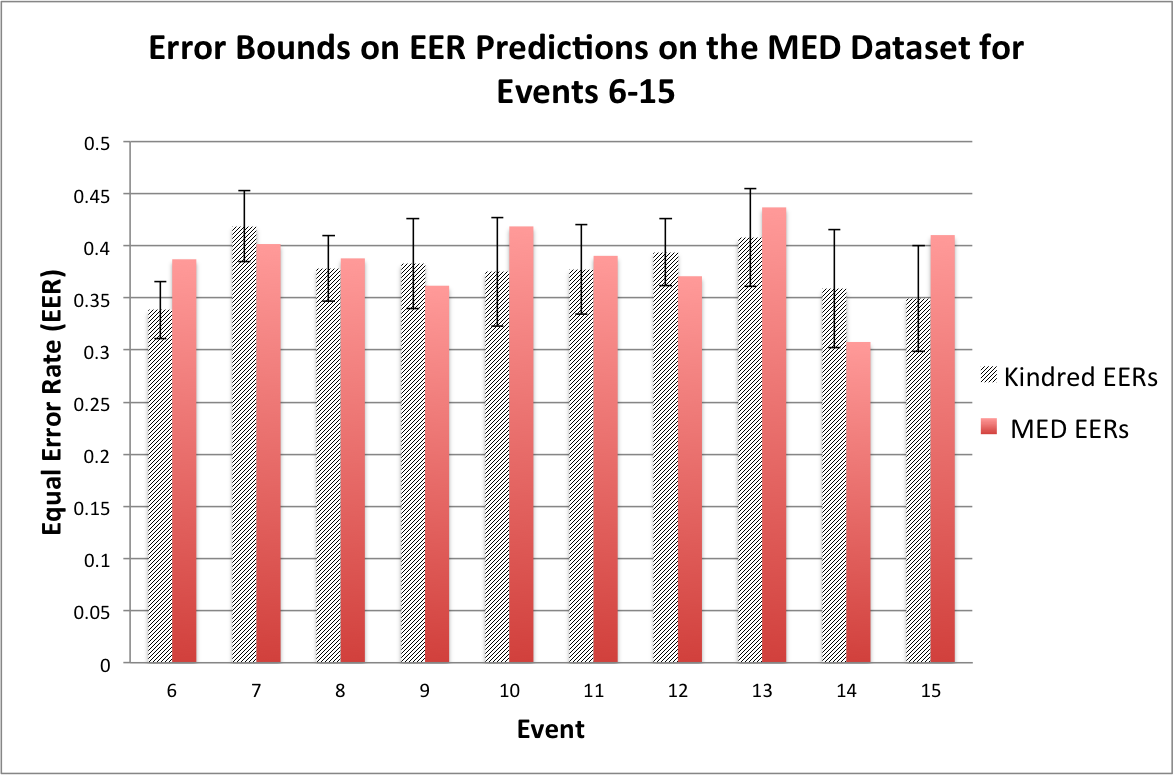
\epsfig{file=figures/errorbounds6-15.png, height=2.0 in, width=3.3in}
\label{fig:blb1}}
\subfigure[Events 21-30]{
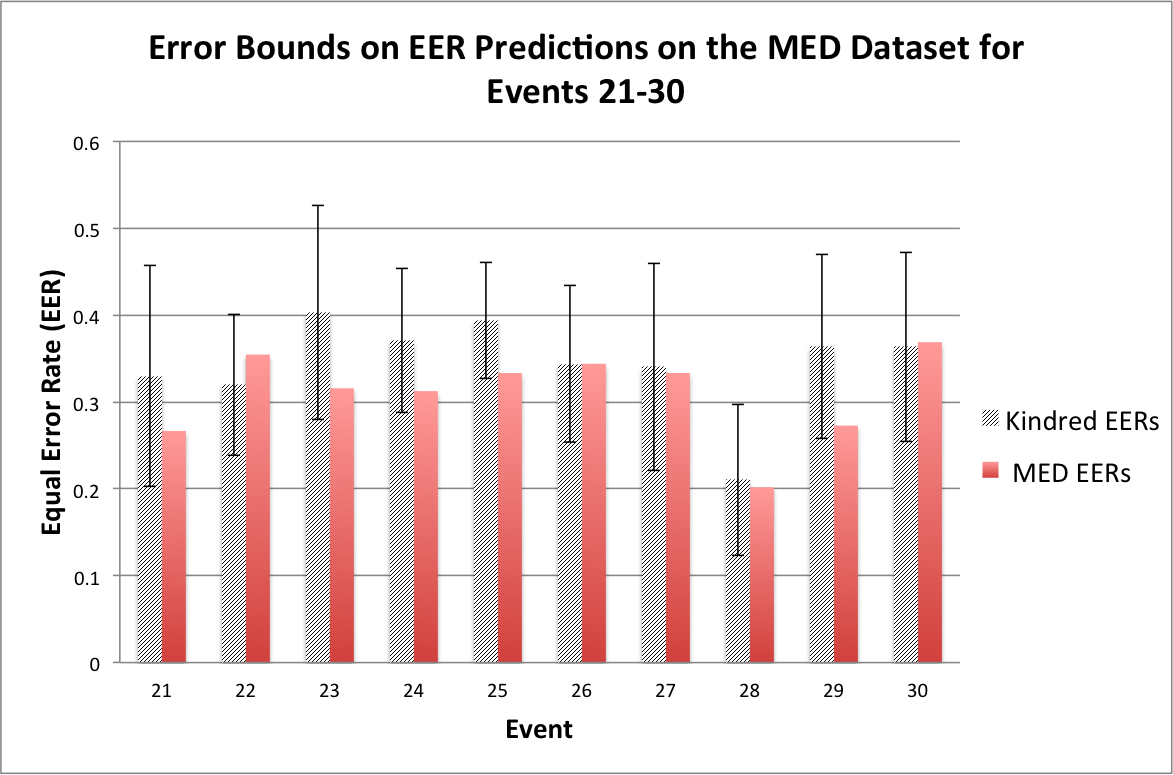
\epsfig{file=figures/errorbounds21-30.png, height=2.0 in, width=3.3in}
\label{fig:blb2}}
\caption{The performance of the video detection system on the Kindred and MED datasets. 
 The error bars display the BLB standard deviations that estimate the variance on the MED dataset from the performance on the Kindred dataset.}
\label{fig:blb}
\end{figure}


\subsection{Comparison to Na\"ive Python}
\begin{figure}
\centering
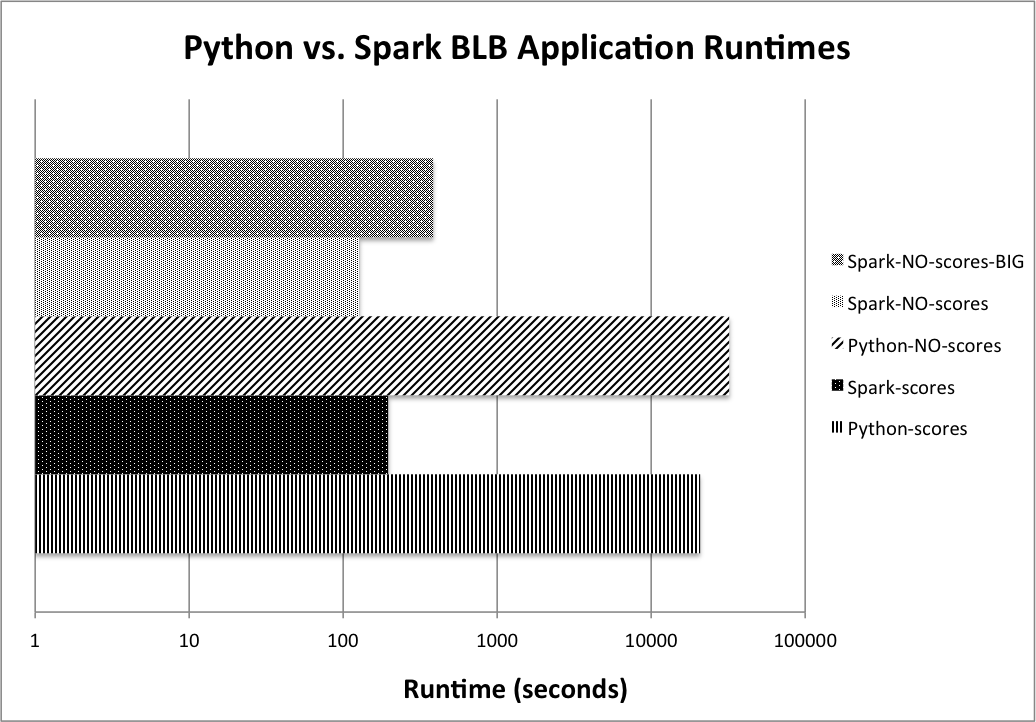
\epsfig{file=figures/pythoncompare.png, height=1.9in, width=3.3in}
\caption{Comparison of runtimes of native Python and generated Spark code. The Spark code, finishing in less than 7 minutes achieves more than a 2 order of magnitude speedup over the 5+ hour Python times. The largest bar is the extrapolated runtime of Python on the BLB application that computes the scores with 100 times more bootstraps to compute than it we test with.}
\label{fig:python}
\end{figure}
 
 As seen in Figure \ref{fig:python}, the Spark code achieves more than a two order of magnitude speedup over the Python code, for both BLB applications tested. The Python code requires an average of 20681 seconds (5.74 hours) and 32142 seconds (8.93 hours) to run when given scores and when not, respectively, whereas the Spark code requires an average of 197.14 seconds (3.29 minutes) and 127.74 seconds (2.13 minutes) to run when given scores and when not, respectively. 
 We can extrapolate runtimes for the BLB application that computes the scores for larger applications. Increasing the number of subsamples and bootstraps up to 20 and 50, respectively, results in 100 (10*10) times more estimates on bootstraps that need to be computed. A 100-fold increase in runtime would amount to a total runtime of 892 hours, likely longer than a researcher's patience would last. 

However, the generated Spark code completes in under 7 minutes, nearly 4 orders of magnitude better than the extrapolated Python runtime. The generated code performs better here relatively since the increased computational load supports a far greater degree of parallelism, whereas on the smaller computation with only 2 subsamples and 5 bootstraps, the need for only 10 bootstrap estimates severly caps the maximum paralellism. This trend of the generated code increasingly outperforming the Python code as the bootstrap computations needed and input data size increase would presumably remain true with more taxing applications since the generated code can simply run on more and more nodes to accomodate the higher demand. 





\section{Future Work}

\section{Conclusion}

Our proposed methodology makes accessible to multimedia classification researchers coding in Python what was never accessible before: an efficient means to estimate video detection system performance via bootstrapping.
This newfound accessibility to efficiency becomes critical on increasingly large consumer-produced multimedia datasets, as we demonstrate. 
With the aid of this methodology, the construction and improvement of video detection systems are made more feasible.






\section{Acknowledgements}


Research supported by Microsoft (Award \#024263) and Intel (Award \#024894) funding and by matching funding by U.C. Discovery (Award \#DIG07-10227). 
Additional support comes from Par Lab affiliates Nokia, NVIDIA, Oracle, and Samsung. Research also funded by DARPA Award Number HR0011-12-2-0016. 



\bibliographystyle{abbrv}

\bibliography{main}

\balancecolumns

\end{document}
